% !TeX spellcheck = it_IT
\newpage
\section{Kubernetes}
Kubernetes è un \textbf{orchestratore} di container. In pratica si assicura che gruppi di container che devono lavorare assieme lo facciano in maniera corretta ed efficiente (un po' come il direttore d'orchestra dà le istruzioni ai musicisti).\\
Si occupa dell'intero \textbf{ciclo di vita} del container, dall'\textit{allocazione} di risorse allo \textit{spegnimento}, nonché della \textit{comunicazione} tra container e della \textit{schedule} ottimale per completare un lavoro.
\subsection{Funzionamento}
La struttura di un sistema con Kubernetes si compone di un \textbf{orchestratore} che espone delle \textbf{API} e che è connesso con molteplici \textbf{worker}, ognuno dei quali è un container a sé stante con un \textbf{kubelet}, ovvero un processo che si occupa di comunicare con l'esterno l'orchestratore.\\
All'orchestratore viene data in pasto una configurazione che rappresenta lo \textbf{stato desiderato}, e lui poi farà in modo, con le risorse che possiede, di mantenerla sempre attiva. Questa configurazione contiene principalmente:
\begin{itemize}
	\item \textbf{Deployment}
	\item \textbf{Pod}: unità più piccola che può contenere una o più immagini di container e della quale si deve specificare il numero di istanze necessarie
\end{itemize}
Nel momento in cui un worker smette di funzionare, l'orchestratore sposta i pod che vi erano in esecuzione su un altro worker, in modo da mantenere costante il numero di repliche attive.
\subsection{Principi}
\subsubsection{Dichiaratività}
Dichiariamo lo \textbf{stato desiderato} del sistema e lasciamo che Kubernetes si occupi di fare tutto ciò che è necessario per raggiungere quell'obiettivo e risolvere eventuali problemi che possono presentarsi.\\
Lo stato desiderato lo definiamo tramite degli \textbf{oggetti}, ognuno con delle specifiche che forniscono lo stato desiderato e lo stato attuale. Kubernetes si occupa poi di verificare costantemente che lo stato attuale sia equivalente a quello desiderato e, in caso non lo sia, provare a ripararlo o sostituirlo direttamente con uno nuovo.
\subsubsection{Distribuzione}
Kubernetes fornisce un'interfaccia unificata per interagire con un cluster di macchine, evitandoci di doverci preoccupare della comunicazione con le singole.
\begin{center}
	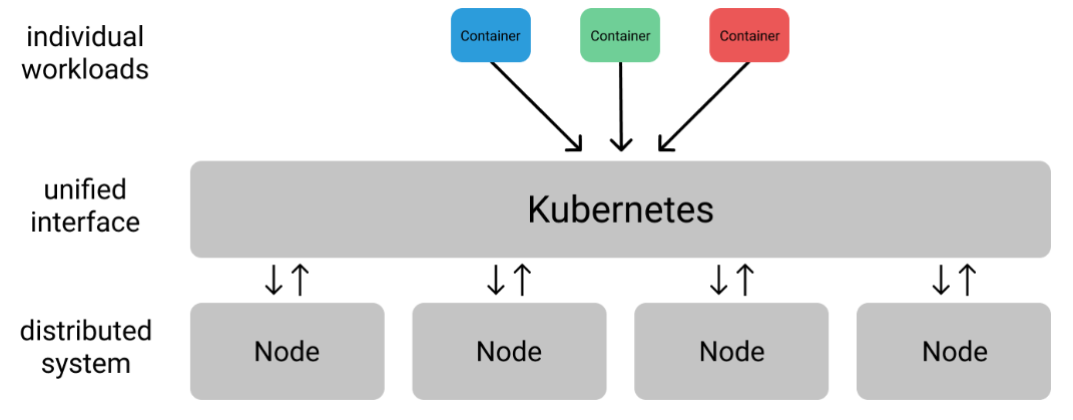
\includegraphics[scale=0.3]{kubernetes_distribution.png}
\end{center}
\subsubsection{Decoupling}
I container devono essere sviluppati in modo che abbiano un singolo compito da svolgere, seguendo i principi dei \textbf{microservizi}.
\subsubsection{Infrastruttura immutabile}
Per ottenere i maggiori benefici dall'orchestrazione di container dobbiamo lavorare basandoci sul principio di un'infrastruttura immutabile. Ad esempio invece di aggiornare eventuali librerie di un container, distruggerlo e ricrearlo da zero con gli aggiornamenti già pronti.\\
Di conseguenza durante l'intero ciclo di vita di un container dobbiamo utilizzare la stessa configurazione ed eventualmente sostituirli con nuovi. \\
Tutto questo ci permette di rendere molto semplice il rollback ad una vecchia versione.
\subsection{Oggetti}
Esistono molti oggetti in Kubernetes, noi ne vedremo solo i principali.
\subsubsection{Manifesto}
Il \textbf{manifesto} contiene la definizione degli oggetti di Kubernetes ed è scritto in \textit{YAML} o \textit{JSON}. Ogni oggetto ha le seguenti informazioni:
\begin{itemize}
	\item Che \textbf{API} usa e quale versione
	\item Che \textbf{tipo} di oggetto è
	\item Cosa \textbf{identifica} in maniera univoca l'oggetto
	\item Lo \textbf{stato} che deve avere l'oggetto
\end{itemize}

\subsubsection{Pod}
Un \textbf{pod} consiste in un insieme di uno o più \textit{container}, un livello \textbf{network} condiviso e volumi del \textbf{filesystem} condivisi.
\subsubsection{Deployment}
Un oggetto di tipo \textbf{deployment} contiene una raccolta di \textit{Pod} definiti da un template e il numero di \textbf{repliche} necessarie per ognuno di essi. Il cluster cercherà in ogni modo di mantenere attive le $n$ repliche indicate del template.
\begin{lstlisting}[style=yaml]
	apiVersion: apps/v1
	kind: Deployment
	metadata:
		name: ml-model-serving
		labels:
			app: ml-model
	spec:
		replicas: 10
		selector:
			matchLabels:
				app: ml-model
		template:
			metadata:
				labels:
					app: ml-model
			spec:
				containers:
				-  name: ml-rest-server
					image: ml-serving:1.0
					ports:
					-  containerPort: 80
\end{lstlisting}
\newpage
\subsubsection{Service}
Ogni \textit{pod} ha un indirizzo IP assegnato che viene usato per la comunicazione. Data la volatilità dei pod, che possono cessare di esistere o essere sostituiti velocemente, l'oggetto \textbf{service} fa il lavoro sporco del capire chi contattare, esponendo all'utente solo degli \textit{endpoint}. Per farlo si basa sulle \textbf{labels}.
\begin{lstlisting}[style=yaml]
	apiVersion: v1
	kind: Service
	metadata:
		name: ml-model-svc
		labels:
			app: ml-model
	spec:
		type: ClusterIP
		selector:
			app: ml-model
		ports:
		-  protocol: TCP
			port: 80
\end{lstlisting}

\subsubsection{Ingress}
Se \textit{Service} permette la comunicazione tramite un unico endpoint nella traffico locale, \textbf{ingress} permette la comunicazione con l'esterno.
\begin{lstlisting}[style=yaml]
	apiVersion: networking.k8s.io/v1beta1
	kind: Ingress
	metadata:
		name: ml-product-ingress
		annotations:
			kubernetes.io/ingress.class: "nginx"
			nginx.ingress.kubernetes.io/rewrite-target: /
	spec:
		rules:
		-  http:
				paths:
				-  path: /app
					backend:
						serviceName: user-interface-svc
						servicePort: 80
\end{lstlisting}
\newpage
\subsection{Control plane}
In un sistema di Kubernetes abbiamo due tipi di macchine:
\begin{itemize}
	\item \textbf{Master node}: spesso singola, contiene la maggior parte dei componenti del pannello di controllo
	\item \textbf{Worker node}: macchina che esegue i workflow dell'applicazione
\end{itemize}

\subsubsection{Master node}
Si compone di:
\begin{itemize}
	\item Il \textbf{server API} convalida la richiesta e fornisce le informazioni sullo stato del cluster, che è salvato in uno storage distribuito di tipo chiave-valore chiamato \textbf{ectd}.\\
	Lo stato contiene diverse informazioni tra cui la configurazione attuale, le specifiche degli oggetti, i loro stati, i nodi presenti e che lavori hanno assegnati.
	\begin{center}
		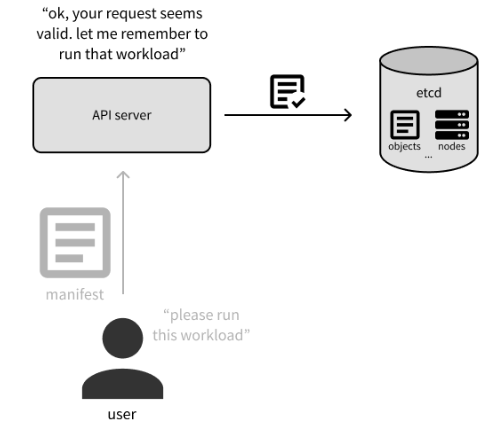
\includegraphics[scale=0.3]{api_server.png}
	\end{center}
	\item Lo \textbf{scheduler} si occupa di decidere su che nodo far partire un determinato workload richiesto:
	\begin{enumerate}
		\item Chiede al \textit{server API} quali oggetti non sono stati assegnati a delle macchine
		\item Determina a quali macchine dovrebbero essere assegnati
		\item Risponde al \textit{server API} comunicandogli gli assegnamenti eseguiti
	\end{enumerate}
	\begin{center}
		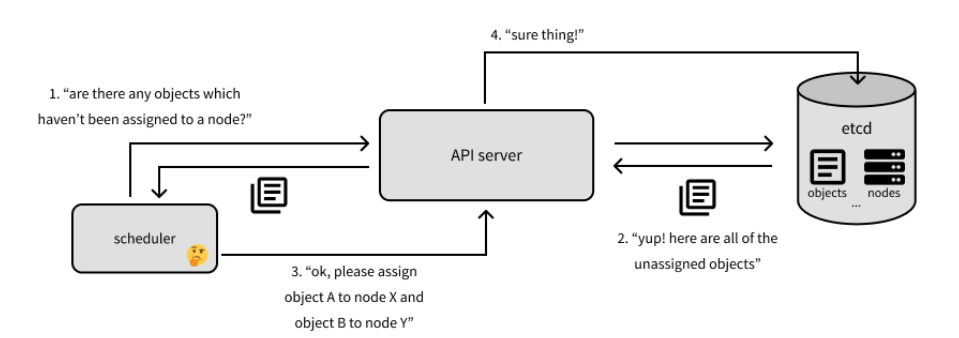
\includegraphics[scale=0.3]{scheduler.png}
	\end{center}
	\item Il \textbf{controller manager} monitora lo stato del cluster attraverso il \textit{server API}. Se lo stato attuale non è quello desiderato, esegue richieste al server in modo da farlo convergere a quello voluto
	\begin{center}
		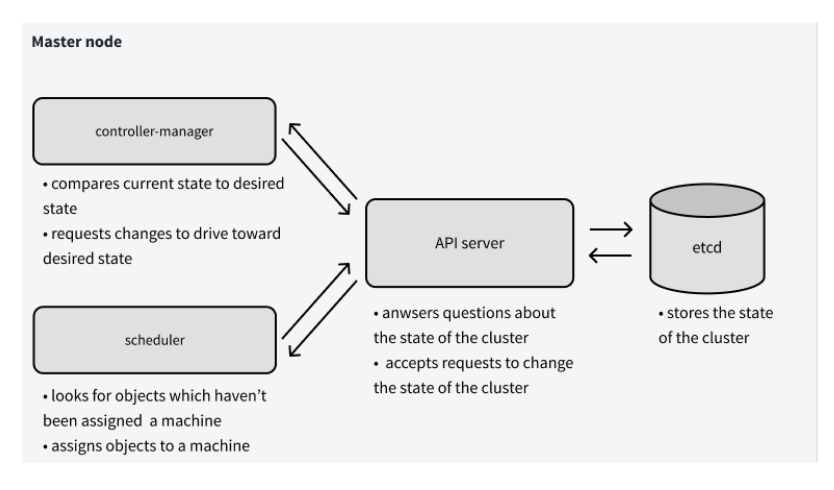
\includegraphics[scale=0.3]{controller_manager.png}
	\end{center}
\end{itemize}
\subsubsection{Worker node}
Il worker node si compone di due elementi:
\begin{itemize}
	\item \textbf{kubelet}: è la parte del nodo che comunica con il \textit{server API}. È responsabile dell'attivazione dei \textit{pod} necessari al workload da eseguire. Appena un nodo entra nel cluster, il \textit{kubelet} lo annuncia al \textit{server API} in modo che lo scheduler possa assegnarli dei workload.
	\begin{center}
		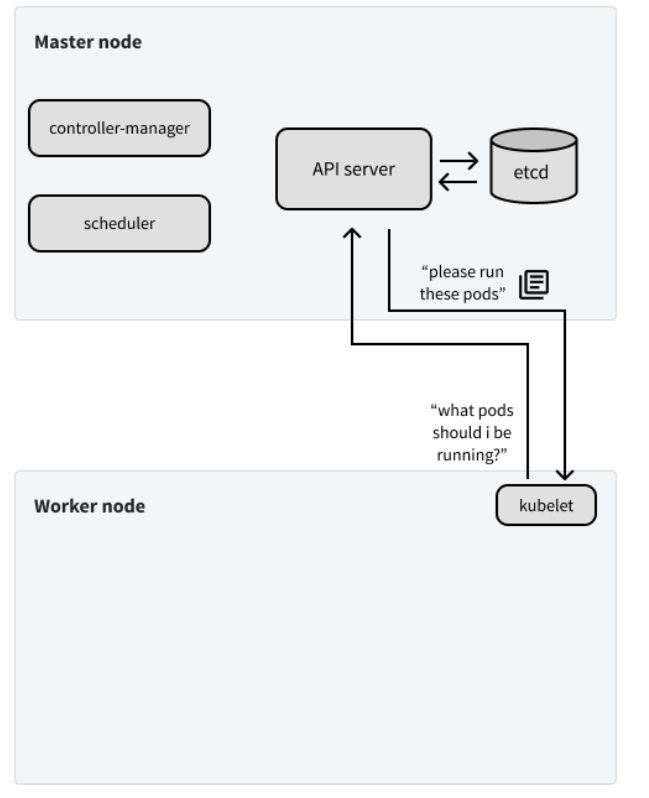
\includegraphics[scale=0.3]{kubelet.png}
	\end{center}
	\item \textbf{kube-proxy}: permette ai container di comunicare tra di loro attraverso i nodi del cluster.
\end{itemize}

\subsection{Conclusione}
Kubernetes non va usato quando:
\begin{itemize}
	\item Il lavoro è leggero e può essere eseguito su una sola macchina
	\item Non è necessario che il servizio sia sempre disponibile
	\item Non sono previste molte modifiche
	\item È progettato in maniera \textit{monolitica}
\end{itemize}
In questi casi è infatti più comodo e veloce usare \textbf{Docker swarm}.